% Created by tikzDevice version 0.12.6 on 2026-10-17 03:42:33
% !TEX encoding = UTF-8 Unicode
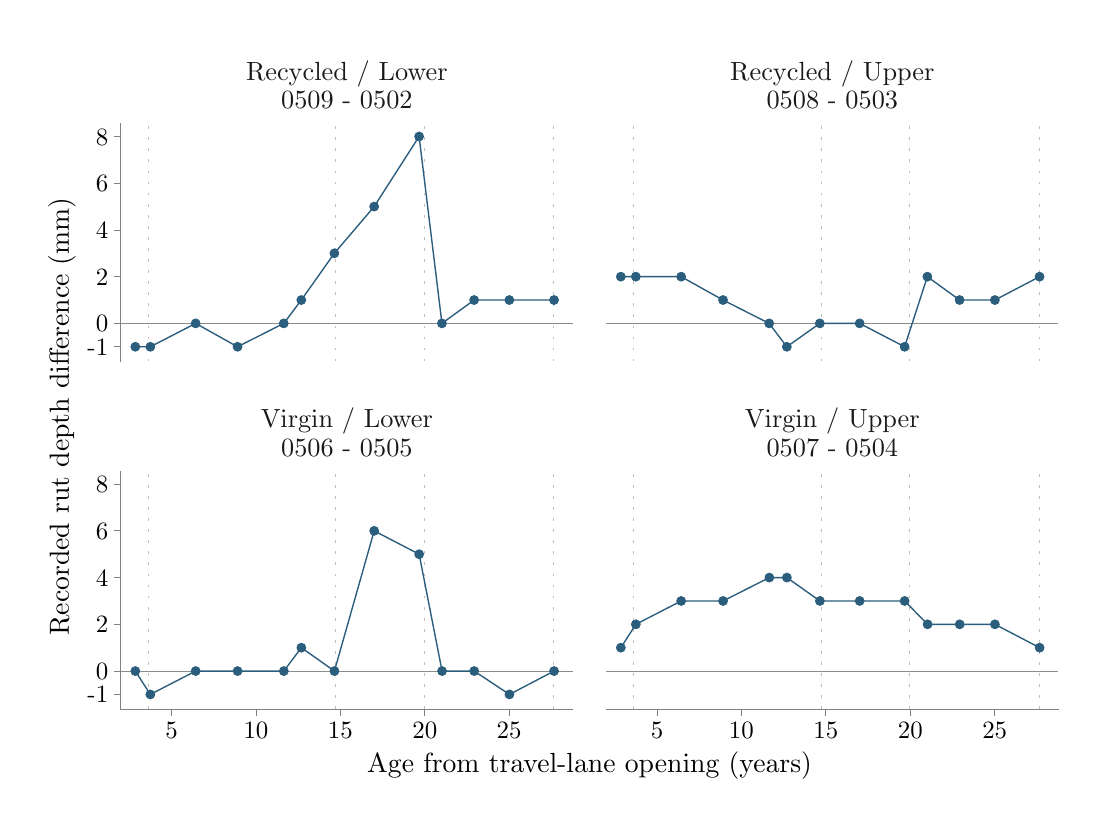
\begin{tikzpicture}[x=1pt,y=1pt]
\definecolor{fillColor}{RGB}{255,255,255}
\path[use as bounding box,fill=fillColor,fill opacity=0.00] (0,0) rectangle (384.48,278.24);
\begin{scope}
\path[clip] (  0.00,  0.00) rectangle (384.48,278.24);
\definecolor{drawColor}{RGB}{255,255,255}
\definecolor{fillColor}{RGB}{255,255,255}

\path[draw=drawColor,line width= 0.5pt,line join=round,line cap=round,fill=fillColor] (  0.00,  0.00) rectangle (384.48,278.24);
\end{scope}
\begin{scope}
\path[clip] ( 33.61,157.61) rectangle (197.04,243.48);
\definecolor{fillColor}{RGB}{255,255,255}

\path[fill=fillColor] ( 33.61,157.61) rectangle (197.04,243.48);
\definecolor{drawColor}{gray}{0.55}

\path[draw=drawColor,line width= 0.3pt,line join=round] ( 33.61,171.38) -- (197.04,171.38);
\definecolor{drawColor}{gray}{0.75}

\path[draw=drawColor,line width= 0.3pt,dash pattern=on 1pt off 3pt ,line join=round] ( 43.48,157.61) -- ( 43.48,243.48);

\path[draw=drawColor,line width= 0.3pt,dash pattern=on 1pt off 3pt ,line join=round] (111.28,157.61) -- (111.28,243.48);

\path[draw=drawColor,line width= 0.3pt,dash pattern=on 1pt off 3pt ,line join=round] (143.25,157.61) -- (143.25,243.48);

\path[draw=drawColor,line width= 0.3pt,dash pattern=on 1pt off 3pt ,line join=round] (190.07,157.61) -- (190.07,243.48);
\definecolor{drawColor}{RGB}{43,93,125}

\path[draw=drawColor,line width= 0.5pt,line join=round] ( 38.90,162.93) --
	( 44.32,162.93) --
	( 60.70,171.38) --
	( 75.83,162.93) --
	( 92.54,171.38) --
	( 98.88,179.82) --
	(110.82,196.71) --
	(125.20,213.59) --
	(141.44,238.92) --
	(149.69,171.38) --
	(161.32,179.82) --
	(174.06,179.82) --
	(190.20,179.82);
\definecolor{fillColor}{RGB}{43,93,125}

\path[draw=drawColor,line width= 0.3pt,line join=round,line cap=round,fill=fillColor] ( 38.90,162.93) circle (  1.61);

\path[draw=drawColor,line width= 0.3pt,line join=round,line cap=round,fill=fillColor] ( 44.32,162.93) circle (  1.61);

\path[draw=drawColor,line width= 0.3pt,line join=round,line cap=round,fill=fillColor] ( 60.70,171.38) circle (  1.61);

\path[draw=drawColor,line width= 0.3pt,line join=round,line cap=round,fill=fillColor] ( 75.83,162.93) circle (  1.61);

\path[draw=drawColor,line width= 0.3pt,line join=round,line cap=round,fill=fillColor] ( 92.54,171.38) circle (  1.61);

\path[draw=drawColor,line width= 0.3pt,line join=round,line cap=round,fill=fillColor] ( 98.88,179.82) circle (  1.61);

\path[draw=drawColor,line width= 0.3pt,line join=round,line cap=round,fill=fillColor] (110.82,196.71) circle (  1.61);

\path[draw=drawColor,line width= 0.3pt,line join=round,line cap=round,fill=fillColor] (125.20,213.59) circle (  1.61);

\path[draw=drawColor,line width= 0.3pt,line join=round,line cap=round,fill=fillColor] (141.44,238.92) circle (  1.61);

\path[draw=drawColor,line width= 0.3pt,line join=round,line cap=round,fill=fillColor] (149.69,171.38) circle (  1.61);

\path[draw=drawColor,line width= 0.3pt,line join=round,line cap=round,fill=fillColor] (161.32,179.82) circle (  1.61);

\path[draw=drawColor,line width= 0.3pt,line join=round,line cap=round,fill=fillColor] (174.06,179.82) circle (  1.61);

\path[draw=drawColor,line width= 0.3pt,line join=round,line cap=round,fill=fillColor] (190.20,179.82) circle (  1.61);
\end{scope}
\begin{scope}
\path[clip] ( 33.61, 31.99) rectangle (197.04,117.86);
\definecolor{fillColor}{RGB}{255,255,255}

\path[fill=fillColor] ( 33.61, 31.99) rectangle (197.04,117.86);
\definecolor{drawColor}{gray}{0.55}

\path[draw=drawColor,line width= 0.3pt,line join=round] ( 33.61, 45.75) -- (197.04, 45.75);
\definecolor{drawColor}{gray}{0.75}

\path[draw=drawColor,line width= 0.3pt,dash pattern=on 1pt off 3pt ,line join=round] ( 43.48, 31.99) -- ( 43.48,117.86);

\path[draw=drawColor,line width= 0.3pt,dash pattern=on 1pt off 3pt ,line join=round] (111.28, 31.99) -- (111.28,117.86);

\path[draw=drawColor,line width= 0.3pt,dash pattern=on 1pt off 3pt ,line join=round] (143.25, 31.99) -- (143.25,117.86);

\path[draw=drawColor,line width= 0.3pt,dash pattern=on 1pt off 3pt ,line join=round] (190.07, 31.99) -- (190.07,117.86);
\definecolor{drawColor}{RGB}{43,93,125}

\path[draw=drawColor,line width= 0.5pt,line join=round] ( 38.90, 45.75) --
	( 44.32, 37.31) --
	( 60.70, 45.75) --
	( 75.85, 45.75) --
	( 92.56, 45.75) --
	( 98.89, 54.20) --
	(110.84, 45.75) --
	(125.21, 96.41) --
	(141.46, 87.97) --
	(149.74, 45.75) --
	(161.34, 45.75) --
	(174.08, 37.31) --
	(190.21, 45.75);
\definecolor{fillColor}{RGB}{43,93,125}

\path[draw=drawColor,line width= 0.3pt,line join=round,line cap=round,fill=fillColor] ( 38.90, 45.75) circle (  1.61);

\path[draw=drawColor,line width= 0.3pt,line join=round,line cap=round,fill=fillColor] ( 44.32, 37.31) circle (  1.61);

\path[draw=drawColor,line width= 0.3pt,line join=round,line cap=round,fill=fillColor] ( 60.70, 45.75) circle (  1.61);

\path[draw=drawColor,line width= 0.3pt,line join=round,line cap=round,fill=fillColor] ( 75.85, 45.75) circle (  1.61);

\path[draw=drawColor,line width= 0.3pt,line join=round,line cap=round,fill=fillColor] ( 92.56, 45.75) circle (  1.61);

\path[draw=drawColor,line width= 0.3pt,line join=round,line cap=round,fill=fillColor] ( 98.89, 54.20) circle (  1.61);

\path[draw=drawColor,line width= 0.3pt,line join=round,line cap=round,fill=fillColor] (110.84, 45.75) circle (  1.61);

\path[draw=drawColor,line width= 0.3pt,line join=round,line cap=round,fill=fillColor] (125.21, 96.41) circle (  1.61);

\path[draw=drawColor,line width= 0.3pt,line join=round,line cap=round,fill=fillColor] (141.46, 87.97) circle (  1.61);

\path[draw=drawColor,line width= 0.3pt,line join=round,line cap=round,fill=fillColor] (149.74, 45.75) circle (  1.61);

\path[draw=drawColor,line width= 0.3pt,line join=round,line cap=round,fill=fillColor] (161.34, 45.75) circle (  1.61);

\path[draw=drawColor,line width= 0.3pt,line join=round,line cap=round,fill=fillColor] (174.08, 37.31) circle (  1.61);

\path[draw=drawColor,line width= 0.3pt,line join=round,line cap=round,fill=fillColor] (190.21, 45.75) circle (  1.61);
\end{scope}
\begin{scope}
\path[clip] (209.04,157.61) rectangle (372.48,243.48);
\definecolor{fillColor}{RGB}{255,255,255}

\path[fill=fillColor] (209.04,157.61) rectangle (372.48,243.48);
\definecolor{drawColor}{gray}{0.55}

\path[draw=drawColor,line width= 0.3pt,line join=round] (209.04,171.38) -- (372.48,171.38);
\definecolor{drawColor}{gray}{0.75}

\path[draw=drawColor,line width= 0.3pt,dash pattern=on 1pt off 3pt ,line join=round] (218.92,157.61) -- (218.92,243.48);

\path[draw=drawColor,line width= 0.3pt,dash pattern=on 1pt off 3pt ,line join=round] (286.71,157.61) -- (286.71,243.48);

\path[draw=drawColor,line width= 0.3pt,dash pattern=on 1pt off 3pt ,line join=round] (318.68,157.61) -- (318.68,243.48);

\path[draw=drawColor,line width= 0.3pt,dash pattern=on 1pt off 3pt ,line join=round] (365.50,157.61) -- (365.50,243.48);
\definecolor{drawColor}{RGB}{43,93,125}

\path[draw=drawColor,line width= 0.5pt,line join=round] (214.34,188.26) --
	(219.75,188.26) --
	(236.14,188.26) --
	(251.27,179.82) --
	(267.94,171.38) --
	(274.32,162.93) --
	(286.24,171.38) --
	(300.63,171.38) --
	(316.88,162.93) --
	(325.10,188.26) --
	(336.75,179.82) --
	(349.50,179.82) --
	(365.65,188.26);
\definecolor{fillColor}{RGB}{43,93,125}

\path[draw=drawColor,line width= 0.3pt,line join=round,line cap=round,fill=fillColor] (214.34,188.26) circle (  1.61);

\path[draw=drawColor,line width= 0.3pt,line join=round,line cap=round,fill=fillColor] (219.75,188.26) circle (  1.61);

\path[draw=drawColor,line width= 0.3pt,line join=round,line cap=round,fill=fillColor] (236.14,188.26) circle (  1.61);

\path[draw=drawColor,line width= 0.3pt,line join=round,line cap=round,fill=fillColor] (251.27,179.82) circle (  1.61);

\path[draw=drawColor,line width= 0.3pt,line join=round,line cap=round,fill=fillColor] (267.94,171.38) circle (  1.61);

\path[draw=drawColor,line width= 0.3pt,line join=round,line cap=round,fill=fillColor] (274.32,162.93) circle (  1.61);

\path[draw=drawColor,line width= 0.3pt,line join=round,line cap=round,fill=fillColor] (286.24,171.38) circle (  1.61);

\path[draw=drawColor,line width= 0.3pt,line join=round,line cap=round,fill=fillColor] (300.63,171.38) circle (  1.61);

\path[draw=drawColor,line width= 0.3pt,line join=round,line cap=round,fill=fillColor] (316.88,162.93) circle (  1.61);

\path[draw=drawColor,line width= 0.3pt,line join=round,line cap=round,fill=fillColor] (325.10,188.26) circle (  1.61);

\path[draw=drawColor,line width= 0.3pt,line join=round,line cap=round,fill=fillColor] (336.75,179.82) circle (  1.61);

\path[draw=drawColor,line width= 0.3pt,line join=round,line cap=round,fill=fillColor] (349.50,179.82) circle (  1.61);

\path[draw=drawColor,line width= 0.3pt,line join=round,line cap=round,fill=fillColor] (365.65,188.26) circle (  1.61);
\end{scope}
\begin{scope}
\path[clip] (209.04, 31.99) rectangle (372.48,117.86);
\definecolor{fillColor}{RGB}{255,255,255}

\path[fill=fillColor] (209.04, 31.99) rectangle (372.48,117.86);
\definecolor{drawColor}{gray}{0.55}

\path[draw=drawColor,line width= 0.3pt,line join=round] (209.04, 45.75) -- (372.48, 45.75);
\definecolor{drawColor}{gray}{0.75}

\path[draw=drawColor,line width= 0.3pt,dash pattern=on 1pt off 3pt ,line join=round] (218.92, 31.99) -- (218.92,117.86);

\path[draw=drawColor,line width= 0.3pt,dash pattern=on 1pt off 3pt ,line join=round] (286.71, 31.99) -- (286.71,117.86);

\path[draw=drawColor,line width= 0.3pt,dash pattern=on 1pt off 3pt ,line join=round] (318.68, 31.99) -- (318.68,117.86);

\path[draw=drawColor,line width= 0.3pt,dash pattern=on 1pt off 3pt ,line join=round] (365.50, 31.99) -- (365.50,117.86);
\definecolor{drawColor}{RGB}{43,93,125}

\path[draw=drawColor,line width= 0.5pt,line join=round] (214.34, 54.20) --
	(219.76, 62.64) --
	(236.14, 71.08) --
	(251.29, 71.08) --
	(268.00, 79.53) --
	(274.34, 79.53) --
	(286.27, 71.08) --
	(300.64, 71.08) --
	(316.89, 71.08) --
	(325.18, 62.64) --
	(336.79, 62.64) --
	(349.51, 62.64) --
	(365.67, 54.20);
\definecolor{fillColor}{RGB}{43,93,125}

\path[draw=drawColor,line width= 0.3pt,line join=round,line cap=round,fill=fillColor] (214.34, 54.20) circle (  1.61);

\path[draw=drawColor,line width= 0.3pt,line join=round,line cap=round,fill=fillColor] (219.76, 62.64) circle (  1.61);

\path[draw=drawColor,line width= 0.3pt,line join=round,line cap=round,fill=fillColor] (236.14, 71.08) circle (  1.61);

\path[draw=drawColor,line width= 0.3pt,line join=round,line cap=round,fill=fillColor] (251.29, 71.08) circle (  1.61);

\path[draw=drawColor,line width= 0.3pt,line join=round,line cap=round,fill=fillColor] (268.00, 79.53) circle (  1.61);

\path[draw=drawColor,line width= 0.3pt,line join=round,line cap=round,fill=fillColor] (274.34, 79.53) circle (  1.61);

\path[draw=drawColor,line width= 0.3pt,line join=round,line cap=round,fill=fillColor] (286.27, 71.08) circle (  1.61);

\path[draw=drawColor,line width= 0.3pt,line join=round,line cap=round,fill=fillColor] (300.64, 71.08) circle (  1.61);

\path[draw=drawColor,line width= 0.3pt,line join=round,line cap=round,fill=fillColor] (316.89, 71.08) circle (  1.61);

\path[draw=drawColor,line width= 0.3pt,line join=round,line cap=round,fill=fillColor] (325.18, 62.64) circle (  1.61);

\path[draw=drawColor,line width= 0.3pt,line join=round,line cap=round,fill=fillColor] (336.79, 62.64) circle (  1.61);

\path[draw=drawColor,line width= 0.3pt,line join=round,line cap=round,fill=fillColor] (349.51, 62.64) circle (  1.61);

\path[draw=drawColor,line width= 0.3pt,line join=round,line cap=round,fill=fillColor] (365.67, 54.20) circle (  1.61);
\end{scope}
\begin{scope}
\path[clip] ( 33.61,117.86) rectangle (197.04,145.61);
\definecolor{drawColor}{gray}{0.10}

\node[text=drawColor,anchor=base,inner sep=0pt, outer sep=0pt, scale=  0.95] at (115.33,133.60) {Virgin / Lower};

\node[text=drawColor,anchor=base,inner sep=0pt, outer sep=0pt, scale=  0.95] at (115.33,123.34) {0506 - 0505};
\end{scope}
\begin{scope}
\path[clip] (209.04,117.86) rectangle (372.48,145.61);
\definecolor{drawColor}{gray}{0.10}

\node[text=drawColor,anchor=base,inner sep=0pt, outer sep=0pt, scale=  0.95] at (290.76,133.60) {Virgin / Upper};

\node[text=drawColor,anchor=base,inner sep=0pt, outer sep=0pt, scale=  0.95] at (290.76,123.34) {0507 - 0504};
\end{scope}
\begin{scope}
\path[clip] ( 33.61,243.48) rectangle (197.04,271.24);
\definecolor{drawColor}{gray}{0.10}

\node[text=drawColor,anchor=base,inner sep=0pt, outer sep=0pt, scale=  0.95] at (115.33,259.23) {Recycled / Lower};

\node[text=drawColor,anchor=base,inner sep=0pt, outer sep=0pt, scale=  0.95] at (115.33,248.97) {0509 - 0502};
\end{scope}
\begin{scope}
\path[clip] (209.04,243.48) rectangle (372.48,271.24);
\definecolor{drawColor}{gray}{0.10}

\node[text=drawColor,anchor=base,inner sep=0pt, outer sep=0pt, scale=  0.95] at (290.76,259.23) {Recycled / Upper};

\node[text=drawColor,anchor=base,inner sep=0pt, outer sep=0pt, scale=  0.95] at (290.76,248.97) {0508 - 0503};
\end{scope}
\begin{scope}
\path[clip] (  0.00,  0.00) rectangle (384.48,278.24);
\definecolor{drawColor}{gray}{0.50}

\path[draw=drawColor,line width= 0.3pt,line join=round,line cap=rect] ( 33.61, 31.99) --
	(197.04, 31.99);
\end{scope}
\begin{scope}
\path[clip] (  0.00,  0.00) rectangle (384.48,278.24);
\definecolor{drawColor}{gray}{0.50}

\path[draw=drawColor,line width= 0.3pt,line join=round] ( 51.99, 29.49) --
	( 51.99, 31.99);

\path[draw=drawColor,line width= 0.3pt,line join=round] ( 82.49, 29.49) --
	( 82.49, 31.99);

\path[draw=drawColor,line width= 0.3pt,line join=round] (112.99, 29.49) --
	(112.99, 31.99);

\path[draw=drawColor,line width= 0.3pt,line join=round] (143.50, 29.49) --
	(143.50, 31.99);

\path[draw=drawColor,line width= 0.3pt,line join=round] (174.00, 29.49) --
	(174.00, 31.99);
\end{scope}
\begin{scope}
\path[clip] (  0.00,  0.00) rectangle (384.48,278.24);
\definecolor{drawColor}{RGB}{0,0,0}

\node[text=drawColor,anchor=base,inner sep=0pt, outer sep=0pt, scale=  0.90] at ( 51.99, 21.31) {5};

\node[text=drawColor,anchor=base,inner sep=0pt, outer sep=0pt, scale=  0.90] at ( 82.49, 21.31) {10};

\node[text=drawColor,anchor=base,inner sep=0pt, outer sep=0pt, scale=  0.90] at (112.99, 21.31) {15};

\node[text=drawColor,anchor=base,inner sep=0pt, outer sep=0pt, scale=  0.90] at (143.50, 21.31) {20};

\node[text=drawColor,anchor=base,inner sep=0pt, outer sep=0pt, scale=  0.90] at (174.00, 21.31) {25};
\end{scope}
\begin{scope}
\path[clip] (  0.00,  0.00) rectangle (384.48,278.24);
\definecolor{drawColor}{gray}{0.50}

\path[draw=drawColor,line width= 0.3pt,line join=round,line cap=rect] (209.04, 31.99) --
	(372.48, 31.99);
\end{scope}
\begin{scope}
\path[clip] (  0.00,  0.00) rectangle (384.48,278.24);
\definecolor{drawColor}{gray}{0.50}

\path[draw=drawColor,line width= 0.3pt,line join=round] (227.42, 29.49) --
	(227.42, 31.99);

\path[draw=drawColor,line width= 0.3pt,line join=round] (257.92, 29.49) --
	(257.92, 31.99);

\path[draw=drawColor,line width= 0.3pt,line join=round] (288.43, 29.49) --
	(288.43, 31.99);

\path[draw=drawColor,line width= 0.3pt,line join=round] (318.93, 29.49) --
	(318.93, 31.99);

\path[draw=drawColor,line width= 0.3pt,line join=round] (349.44, 29.49) --
	(349.44, 31.99);
\end{scope}
\begin{scope}
\path[clip] (  0.00,  0.00) rectangle (384.48,278.24);
\definecolor{drawColor}{RGB}{0,0,0}

\node[text=drawColor,anchor=base,inner sep=0pt, outer sep=0pt, scale=  0.90] at (227.42, 21.31) {5};

\node[text=drawColor,anchor=base,inner sep=0pt, outer sep=0pt, scale=  0.90] at (257.92, 21.31) {10};

\node[text=drawColor,anchor=base,inner sep=0pt, outer sep=0pt, scale=  0.90] at (288.43, 21.31) {15};

\node[text=drawColor,anchor=base,inner sep=0pt, outer sep=0pt, scale=  0.90] at (318.93, 21.31) {20};

\node[text=drawColor,anchor=base,inner sep=0pt, outer sep=0pt, scale=  0.90] at (349.44, 21.31) {25};
\end{scope}
\begin{scope}
\path[clip] (  0.00,  0.00) rectangle (384.48,278.24);
\definecolor{drawColor}{gray}{0.50}

\path[draw=drawColor,line width= 0.3pt,line join=round,line cap=rect] ( 33.61,157.61) --
	( 33.61,243.48);
\end{scope}
\begin{scope}
\path[clip] (  0.00,  0.00) rectangle (384.48,278.24);
\definecolor{drawColor}{RGB}{0,0,0}

\node[text=drawColor,anchor=base east,inner sep=0pt, outer sep=0pt, scale=  0.90] at ( 29.11,159.84) {-1};

\node[text=drawColor,anchor=base east,inner sep=0pt, outer sep=0pt, scale=  0.90] at ( 29.11,168.29) {0};

\node[text=drawColor,anchor=base east,inner sep=0pt, outer sep=0pt, scale=  0.90] at ( 29.11,185.17) {2};

\node[text=drawColor,anchor=base east,inner sep=0pt, outer sep=0pt, scale=  0.90] at ( 29.11,202.06) {4};

\node[text=drawColor,anchor=base east,inner sep=0pt, outer sep=0pt, scale=  0.90] at ( 29.11,218.95) {6};

\node[text=drawColor,anchor=base east,inner sep=0pt, outer sep=0pt, scale=  0.90] at ( 29.11,235.83) {8};
\end{scope}
\begin{scope}
\path[clip] (  0.00,  0.00) rectangle (384.48,278.24);
\definecolor{drawColor}{gray}{0.50}

\path[draw=drawColor,line width= 0.3pt,line join=round] ( 31.11,162.93) --
	( 33.61,162.93);

\path[draw=drawColor,line width= 0.3pt,line join=round] ( 31.11,171.38) --
	( 33.61,171.38);

\path[draw=drawColor,line width= 0.3pt,line join=round] ( 31.11,188.26) --
	( 33.61,188.26);

\path[draw=drawColor,line width= 0.3pt,line join=round] ( 31.11,205.15) --
	( 33.61,205.15);

\path[draw=drawColor,line width= 0.3pt,line join=round] ( 31.11,222.04) --
	( 33.61,222.04);

\path[draw=drawColor,line width= 0.3pt,line join=round] ( 31.11,238.92) --
	( 33.61,238.92);
\end{scope}
\begin{scope}
\path[clip] (  0.00,  0.00) rectangle (384.48,278.24);
\definecolor{drawColor}{gray}{0.50}

\path[draw=drawColor,line width= 0.3pt,line join=round,line cap=rect] ( 33.61, 31.99) --
	( 33.61,117.86);
\end{scope}
\begin{scope}
\path[clip] (  0.00,  0.00) rectangle (384.48,278.24);
\definecolor{drawColor}{RGB}{0,0,0}

\node[text=drawColor,anchor=base east,inner sep=0pt, outer sep=0pt, scale=  0.90] at ( 29.11, 34.22) {-1};

\node[text=drawColor,anchor=base east,inner sep=0pt, outer sep=0pt, scale=  0.90] at ( 29.11, 42.66) {0};

\node[text=drawColor,anchor=base east,inner sep=0pt, outer sep=0pt, scale=  0.90] at ( 29.11, 59.55) {2};

\node[text=drawColor,anchor=base east,inner sep=0pt, outer sep=0pt, scale=  0.90] at ( 29.11, 76.44) {4};

\node[text=drawColor,anchor=base east,inner sep=0pt, outer sep=0pt, scale=  0.90] at ( 29.11, 93.32) {6};

\node[text=drawColor,anchor=base east,inner sep=0pt, outer sep=0pt, scale=  0.90] at ( 29.11,110.21) {8};
\end{scope}
\begin{scope}
\path[clip] (  0.00,  0.00) rectangle (384.48,278.24);
\definecolor{drawColor}{gray}{0.50}

\path[draw=drawColor,line width= 0.3pt,line join=round] ( 31.11, 37.31) --
	( 33.61, 37.31);

\path[draw=drawColor,line width= 0.3pt,line join=round] ( 31.11, 45.75) --
	( 33.61, 45.75);

\path[draw=drawColor,line width= 0.3pt,line join=round] ( 31.11, 62.64) --
	( 33.61, 62.64);

\path[draw=drawColor,line width= 0.3pt,line join=round] ( 31.11, 79.53) --
	( 33.61, 79.53);

\path[draw=drawColor,line width= 0.3pt,line join=round] ( 31.11, 96.41) --
	( 33.61, 96.41);

\path[draw=drawColor,line width= 0.3pt,line join=round] ( 31.11,113.30) --
	( 33.61,113.30);
\end{scope}
\begin{scope}
\path[clip] (  0.00,  0.00) rectangle (384.48,278.24);
\definecolor{drawColor}{RGB}{0,0,0}

\node[text=drawColor,anchor=base,inner sep=0pt, outer sep=0pt, scale=  1.00] at (203.04,  9.13) {Age from travel-lane opening (years)};
\end{scope}
\begin{scope}
\path[clip] (  0.00,  0.00) rectangle (384.48,278.24);
\definecolor{drawColor}{RGB}{0,0,0}

\node[text=drawColor,rotate= 90.00,anchor=base,inner sep=0pt, outer sep=0pt, scale=  1.00] at ( 14.87,137.74) {Recorded rut depth difference (mm)};
\end{scope}
\end{tikzpicture}
